\documentclass{article}

\usepackage{amsmath}
\usepackage{amssymb}
\usepackage{amsfonts}
\usepackage{amsthm}
\usepackage{amsrefs}

\usepackage{graphicx}
\usepackage{caption}
\usepackage{subcaption}

\usepackage[margin=0.5in]{geometry}

\usepackage[spanish, mexico]{babel}

\usepackage[utf8]{inputenc}

\title{Deducción de la Ecuación de Calor en 3 Dimensiones.}
\author{Miguel A. Gomez B.}

\begin{document}
\maketitle

\subparagraph{Abstract}\textit{The abstract}

\section*{Introducción}
\paragraph{}¿Son las matemáticas la estructura que describe la naturaleza? Si bien aún hoy en día es debatible la respuesta de esta pregunta, personajes como Galileo, Newton o Fourier, nos han demostrado con sus trabajos, que las matemáticas y específicamente: El cálculo, es un lenguaje muy cercano a la realidad. Uno de estos fenómenos es el de la difusión del calor, estudiado con gran interés por Joseph Fourier. En este artículo pretendo explicar algunas de las ideas que permitieron la construcción del modelo que describe el fenómeno físico, resaltando algunos personajes o temas de interés general en el modelamiento de este tipo de sistemas.
\begin{center}
	------------
\end{center}
\section{Preliminares}
\paragraph{} Cuando Isaac Newton encontró una explicación matemática de las órbitas planetarias, en realidad estaba resolviendo un problema de \textit{ecuaciones diferenciales ordinarias} (que sea ordinaria nos indica que tiene solamente una variable independiente) y en este caso Newton el objeto construido por Newton, fue un modelo descrito con una función de posición respecto al tiempo, que describe el cambio de la posición de un cuerpo momento a momento\footnote{Aquí por momento nos referimos a diferencias de tiempo y de espacio cercanas a cero, es decir infinitesimales.} de acuerdo a lo que dicta la ecuación
$$F=ma,$$
\paragraph{}en general muchos otros modelos son descritos respecto a una variable y el tiempo, los modelos poblacionales por ejemplo, pueden responder a cuántos individuos pueden haber en una población en un tiempo determinado, otros modelan la rapidez con la que se contagia un virus, luego de manera general podemos decir que una ecuación diferencial ordinaria describe el cambio infinitesimal de algo respecto a otro algo que cambia también de manera infinitesimal (como un incremento en el tiempo) y ello es independiente de cuantas variables dependientes tenga, por ejemplo una bala de cañón en 3 dimensiones, podríamos decir que la posición de bala se describe con coordenadas $(x,y,z)$ y modelar funciones $x(t)$, $y(t)$, $z(t)$ que describen el movimiento pero ¿este modelo es consistente con la realidad? que tal si planteáramos en lugar de una bala, ¿el movimiento de un cohete espacial?
\begin{figure}[h!]
  \centering
  \begin{subfigure}[b]{0.2\linewidth}
    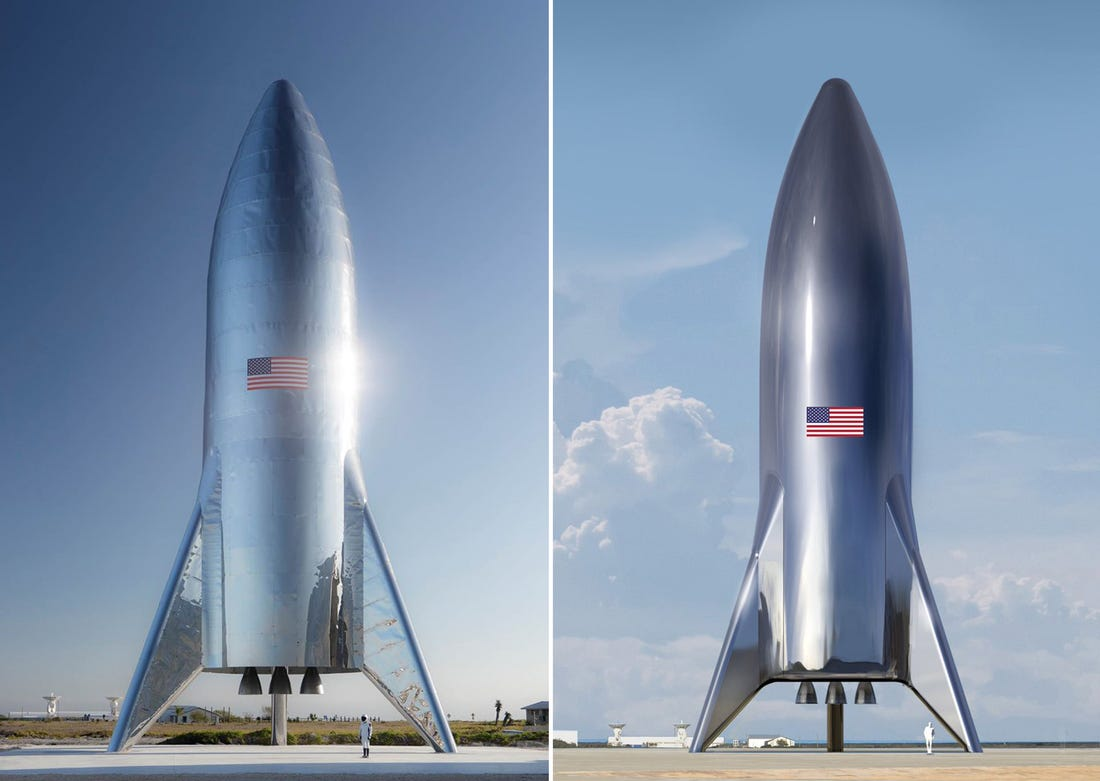
\includegraphics[width=\linewidth]{heat_equation_article/img/rocket.jpg}
  \end{subfigure}
  \begin{subfigure}[b]{0.2\linewidth}
    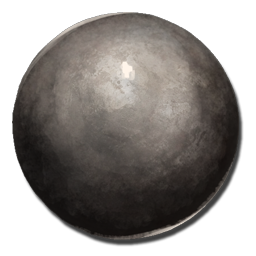
\includegraphics[width=\linewidth]{heat_equation_article/img/Cannon_Ball.png}
  \end{subfigure}
\end{figure}
\paragraph{}Nótese que aunque ambos problemas pretenden encontrar la posición de un objeto respecto al tiempo, en el fondo son problemas muy diferentes, la forma del objeto y los cambios en el medio en el que viaja este objeto y demás factores, van a influir en cómo cambia la posición de este objeto, dicho de otro modo, idealizamos el fenómeno que vamos a estudiar, lo cual nos permite tener una idea mucho mas sencilla (o complicada en algunos casos) de como funciona este fenómeno\footnote{Lo cual no implica que sean modelos con menor validez, algunos modelos de ecuaciones ordinarias aún son utilizados hoy en día para estudiar todo tipo de fenómenos que implican cambio.}
\paragraph{}No todos los sistemas se comportan en la manera de una ecuación diferencial, consideremos otro ejemplo, una tetera recién puesta en la estufa, en estos momentos es conocido que una cantidad de moléculas se encuentran \textit{revoloteando} de manera errática y ello es lo que produce el calor, pero no hay manera de cuantificar (o por lo menos no muy sencilla y práctica) de predecir su movimiento, debido a que es prácticamente impredecible. Sin embargo otra manera de explicar este fenómeno es ver la tetera como un todo y construímos una función $T(x,y,z,t)$, que describirá la temperatura en alguna parte del fluído (mas formalmente, decimos que es contínua), en un tiempo $t$.
\paragraph{} Detengámonos un momento para estructurar un poco mejor la idea detrás, la ley de enfríamiento de Newton nos dice que(traducido de \cite{raymondserway2013}): \textit{El cambio en la pérdida de calor de un cuerpo es directamente proporcional entre el cuerpo y sus alrededores.\footnote{El texto original dice: \textit{the rate of heat loss of a body is directly proportional to the difference in the temperatures between the body and its surroundings.}}} Luego respecto al fenómeno de calor podríamos decir que:
\begin{itemize}
    \item La temperatura puede ser diferente en diferentes partes del cuerpo.
    \item La temperatura de una de estas partes del cuerpo tiene una relación con las otras partes del cuerpo que la rodean.
\end{itemize}
\paragraph{}Parece no ser muy claro, pero recordemos el ejemplo de la tetéra, en el inicio podríamos decir si medimos la temperatura en cualesquiera de las partes del fluído tendríamos una temperatura casi que igual, pero a medida que pase el tiempo veremos que el fluído va a estar mas caliente en el fondo de la tetéra\footnote{O imagine un cubo de hielo sobre una sartén, veremos que empezará a derretirse desde la parte mas baja, es decir en efecto la  ley de Newton es consistente con lo que evidenciamos.}, vemos ahora que a diferencia de las ecuaciones diferenciales ordinarias, tenemos una dependencia no sólo respecto al tiempo, sino también respecto a como cambia la temperatura en las diferentes partes del cuerpo y necesitamos un nuevo objeto para describir matemáticamente las relaciones en este fenómeno, estas son las \textit{ecuaciones diferenciales parciales}.
\paragraph{}Las ecuaciones diferenciales parciales nos permiten modelar sistemas en donde existen cambios simultáneos en el espacio y el tiempo\cite{stevenstrogatz2019}, sin embargo aunque en ciertos casos nos permiten describir este tipo de fenómenos, resolverlas es en general muy difícil.
\section{La llegada de Joseph Fourier}
\begin{center}
\textit{En los 1800, el calor era un acertijo. Se desconocía lo que era exactamente ¿Era como un líquido? parecía 'fluir', pero era imposible sostenerlo con las manos o verlo (...) Los secretos de este fenómeno fueron revelados por un hombre que generalmente sentía frío (...)}\cite{stevenstrogatz2019}.
\end{center}
\begin{center}
    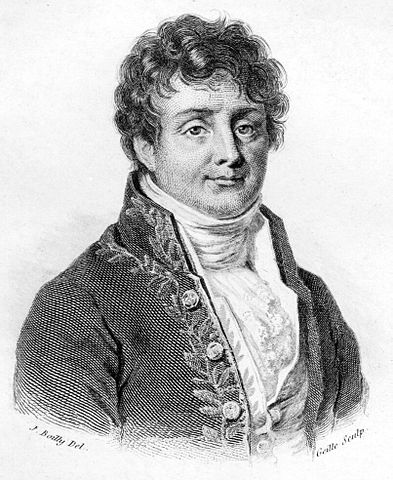
\includegraphics[width=0.2\linewidth]{heat_equation_article/img/393px-Joseph_Fourier.jpg}
\end{center}
\paragraph{}Ese hombre era Jean Baptiste Joseph Fourier (1768-1830). Huérfano desde los 10, Fourier era un niño con problemas de salud. En \cite{Fleming1999} encontramos algunos detalles muy interesantes de este personaje:
\begin{center}
    \textit{Era conocido por sus contemporáneos como un amigo de Napoleón, administrador, egiptólogo, matemático y científico (...) fue un profesor de matemáticas, un policía secreto y (dos veces) prisionero político, gobernador de Egipto y miembro perpetuo y secretario de la Academia Francesa de Ciencias.}
\end{center}
En general, este hombre estaba obsesionado con el calor, todos sus trabajos tienen un interés muy estrecho con el calor, una de sus publicaciones con mayor fama: \textit{ Théorie analytique de la chaleur (1822)}\footnote{Sería Lord Kelvin quien describiría este trabajo de Fourier como 'un gran poema matemático'\cite{Fleming1999}.}, contiene el primer registro de matemáticas que estudian la difusión del calor y fue la primera matematización de una rama de la física fuera de la mecánica, esta obra de Fourier se convierte en la pricipal fuente para las personas que estudian la difusión del calor\footnote{Otro detalle interesante es que en esta obra Fourier no hace ningún compromiso con el comportamiento del calor en la naturaleza, el lo asume como un fenómeno, con el frío como su opuesto \cite{GrattanGuinness2005}}, sin embargo otros estudios previos de Fourier, culminan en su trabajo ‘observaciones generales sobre la temperatura de la tierra y el espacio interplanetario’.
\paragraph{Ideas para el desarrollo del texto}
Warm up: ¿Cómo se representa el cambio? visualmente, geométricamente y algebráicamente (explicación de las ecuaciones).

¿Preguntarse qué función ayuda a resolver el sistema?

Que ocurre cuando hay mayores interacciones.

¿Es una función de posición?

En física es mucho más común utilizar segundo orden.

PDEs: el problema consiste en solucionar un continuo de puntos infinitos (el solido) en el que otras.

La realidad es que utilizamos aproximaciones a la realidad, pero aún así hay restricciones (caos? algo que no medimos?) [Poner un ejemplo, e ir explicando sus propiedades matemáticas, resaltando conclusiones y explicandolas, encontrar cosas contradictorias a la intuición pero que representan la realidad]

Introducción a a solución
Imaginarse la solución de acuerdo a las leyes físicas y cuál sería su comportamiento. Visualizar todas las posibles soluciones, iniciar la Descripción de los parámetros y cómo se relacionan, dar ejemplos y deducciones ¿Cómo cambia en el tiempo? Dar un objeto matemático y cuestionar lo que representa. Luego explicar que es una construcción abstracta.

En la solución hacer cambios de notación para hacer mucho mas familiar el objeto.

¿Es un campo vectorial?

Describir el proceso para solucionarlas (revisar lo de simulación)
Apreciar la dificultad de resolver estas ecuaciones
parece mas un arte que una ciencia (encontrar las soluciones)
Mostrar en que casos puede romperse respecto a la realidad debido a los parámetros que utilizamos.

Comparar la solución con lo que dice la ciencia acerca del fenómeno. Qué pasa si cambiamos parámetros del fenómeno. Hacia qué comportamiento tiende.

Como describimos el fenómeno. Espacio fase. Cuál es la ventaja e utilizar este fenómeno.  Cita de Chaos("... una de las más poderosas invenciones de la ciencia moderna."), explicar la razón (todas las posibilidades de estados, están contenidas)

Visualizar hacia a donde tiende con el gráfico y Verificar matemáticamente el fenómeno.

¿Como se transfiere esto a otros fenómenos?

Finite-steps: explicación.

teoría del Caos, estable, inestable, atractores.

¿Series de fourier para resolver la ecuación?

Otras conexiones con otros objetos y la versatilidad de las matemáticas.

Sabemos que si un valor... caos

'Incluso si logramos entender porqué esto ocurre, hay "semillas" que producen cambios caóticos. Revisando desde el inicio, ... es cruel que el universo sea así, pero nos da esperanza en que la complejidad del mundo puede ser estudiada desde la matemática y no está escondida fuera entre las inconsistencias de nuestros modelos y el fenómeno natural'. 
\nocite{*}
\bibliography{bibliography}
\end{document}